% !TeX root = surprises.tex

%%%%%%%%%%%%%%%%%%%%%%%%%%%%%%%%%%%%%%%%%%%%%%%%%%%%%%%%%%%%%%%%

\selectlanguage{hebrew}

\chapter{האקסיומות של אוריגמי}\label{c.origami-axioms}

אוריגמי, האומנות של קיפולי נייר, פותח לפני מאות שנים ביפן והיום יש לו קהילה בינלאומית. לקראת סוף המאה העשרים, פוחתה התיאוריה המתמטית של אוריגמי שבסיסה שבע אקסיומות, אקסיומות
\L{Huzita–Hatori},
על שם
\L{Humiaki Huzita}
שמצא את ששת האקסיומות הראשונות ו-%
\L{Koshiro Hatori}
שמצא את השביעית.
\L{Jacques Justin}
פירסם את כל שבעת האקסיומות לפני
\L{Huzita}
ו-%
\L{Hatori},
ו-%
\L{Margherita P. Beloch}
הציגה את האקסיומה השישית ב-%
$1936$.
למרות זאת, האקסיומות ידועות כאקסיומות
\L{Huzita-Hatori}.

בסדרה של שלושה פרקים נלמד את המתמטיקה של אוריגמי. פרק זה מציג את האקסיומות, פרק%
~\ref{c.origami-cube}
קושר את אוריגמי עם השורשים של פולינומים ופרק%
~\ref{c.origami-constructions} 
מראה שבניות שאינן אפשריות עם סרגל ומחוגה ניתנות לבנייה עם אוריגמי.
 
פרק זה מכיל סעיף עבור כל אחת מהאקסיומות. לאחר ניסוח האקסיומה ותרשים של 
\textbf{הקיפול}
שהיא מתארת, נפתח את משוואות הקיפול ושל נקודות החיתוך באמצעות גיאומטריה אנליטית. ניתן להגדיר קיפול גם 
\textbf{כמקום הגיאומטרי}
שהוא מתאר, קבוצת כל הנקודות המקיימות תכונה מסויימת. המונח קיפול בא מהפעולה של קיפול דף נייר באוריגמי, אבל כאן הוא משמש לקו הגיאומטרי שנוצר על ידי קיפול הדף.

התוצאה של פעולת הקיפול היא
\textbf{שיקוף}.
נתון נקודה
$p$,
השיקוף שלה סביב הקיפול
$l$
היא הנקודה 
$p'$
כך ש-%
$l$
הוא האנך האמצעי של קטע הקו
$\overline{pp'}$
(איור%
~\ref{f.origami-def}).
\begin{figure}[tb]
\begin{center}
\begin{tikzpicture}[scale=.8]
\coordinate (P1) at (2,2);
\coordinate (P1P) at (6,4);
\coordinate (mid) at (4,3);
\draw[rotate=30] (mid) rectangle +(8pt,8pt);
\coordinate (m1) at ($(P1)!.5!(mid)$);
\coordinate (m2) at ($(mid)!.5!(P1P)$);
\draw[thick] (m1) -- +(120:4pt);
\draw[thick] (m1) -- +(-60:4pt);
\draw[thick] (m2) -- +(120:4pt);
\draw[thick] (m2) -- +(-60:4pt);
\draw[thick] (P1) -- (P1P);
\draw[very thick,dashed] (4.7,1.6) -- node[very near end,right,yshift=4pt] {$l$} (3.5,4);
\vertex{P1};
\vertex{P1P};
\node[above left] at (P1) {$p$};
\node[above left] at (P1P) {$p'$};
\draw[very thick,dotted,->,bend right=50] (2.1,1.9) to (6.05,3.9);
\end{tikzpicture}
\end{center}
\selectlanguage{hebrew}
\caption{הקפל הוא האנך האמצעי של הקו שמחבר בין נקודה לשיקוף שלה}
\label{f.origami-def}
\end{figure}

\section{אקסיומה 1}\label{s.ax1}


\begin{axiom}
נתונות שתי נקודות שונות
$p_1=(x_1,y_1)$, $p_2=(x_2,y_2)$,
קיים קיפול יחיד
$l$
העובר דרך שתיהן (איור%
~\ref{f.axiom1}).
\end{axiom}
\begin{figure}[tb]
\begin{center}
\begin{tikzpicture}[scale=1]
\draw[step=10mm,white!50!black,thin] (-1,-1) grid (8,6);
\draw[thick] (-1,0) -- (8,0);
\draw[thick] (0,-1) -- (0,6);
\foreach \x in {0,...,8}
  \node at (\x-.2,-.2) {\sm{\x}};
\foreach \y in {1,...,6}
  \node at (-.2,\y-.3) {\sm{\y}};
\coordinate (P1) at (2,2);
\coordinate (P2) at (6,4);
\draw[very thick,dashed] ($(P1)!-.75!(P2)$) -- node[very near end,below] {$l$} ($(P1)!1.5!(P2)$);
\vertex{P1};
\vertex{P2};
\node[above left] at (P1) {$p_1$};
\node[above left] at (P2) {$p_2$};

\draw[very thick,dotted,->,bend left=30] (2,5) to (4,1);
\end{tikzpicture}
\end{center}
\selectlanguage{hebrew}
\caption{אקסיומה 1}\label{f.axiom1}
\end{figure}

\textbf{פיתוח משוואת הקיפול:}
השיפוע של הקיפול הוא המנה של הפרשי הקואורינטות של
$p_1,p_2$
ונקדות החיתוך עם ציר ה-%
$y$
מתקבלת מ-%
$p_1$:
\begin{equation}
y - y_1 = \disfrac{y_2-y_1}{x_2-x_1}(x-x_1)\,.
\end{equation}
\begin{example}
נתונות הנקודות
$p_1=(2,2), p_2=(6,4)$,
המשוואה של 
$l$  היא:

\begin{eqn}
y-2&=&\disfrac{4-2}{6-2}(x-2)\\
y&=&\disfrac{1}{2}x+1\,.
\end{eqn}
\end{example}

%%%%%%%%%%%%%%%%%%%%%%%%%%%%%%%%%%%%%%%%%%%%%%%%%%%%%%%%%%%%%%%%

\section{אקסיומה 2}\label{s.ax2}


\begin{axiom}
נתונות שתי נקודות שונות
$p_1=(x_1,y_1)$, $p_2=(x_2,y_2)$,
קיים קיפול יחיד 
$l$
המניח את
$p_1$
על
$p_2$
(איור~%
\ref{f.axiom2}).
\end{axiom}

הקיפול הוא המקום הגיאומטרי של כל הנקודות במרחק שווה מ-%
$p_1$
ו-%
$p_2$.
\begin{figure}[tb]
\begin{center}
\begin{tikzpicture}[scale=1]
\draw[step=10mm,white!50!black,thin] (-1,-1) grid (8,6);
\draw[thick] (-1,0) -- (8,0);
\draw[thick] (0,-1) -- (0,6);
\foreach \x in {0,...,8}
  \node at (\x-.2,-.2) {\sm{\x}};
\foreach \y in {1,...,6}
  \node at (-.2,\y-.3) {\sm{\y}};
\coordinate (P1) at (2,2);
\coordinate (P2) at (6,4);
\coordinate (mid1) at ($(P1)!.5!(P2)$);
\coordinate (mid2) at ($(P1)!.5!(P2)+(-1,2)$);

\draw[rotate=30] (mid1) rectangle +(8pt,8pt);

\draw (P1) -- (P2);
\draw[very thick,dashed] ($(mid1)!-1.4!(mid2)$) -- node[very near end,left,yshift=-12pt] {$l$} ($(mid1)!1.4!(mid2)$);
\vertex{P1};
\vertex{P2};
\node[above left] at (P1) {$p_1$};
\node[above left] at (P2) {$p_2$};

\draw[very thick,dotted,->,bend right=50] (2.1,1.9) to (6,3.9);
\end{tikzpicture}
\caption{אקסיומה 2}\label{f.axiom2}
\end{center}
\end{figure}


\textbf{פיתוח משוואת הקיפול:}
הקיפול 
$l$
הוא האנך האמצעי של
$\overline{p_1p_2}$.
השיפוע שלו הוא ההופכי השלילי של השיפוע של הקו המחבר את
$p_1$
ו-%
$p_2$.
$l$
עובר דרך נקודת האמצע בין שתי הנוקדות:
\begin{equation}
y - \disfrac{y_1+y_2}{2} = -\disfrac{x_2-x_1}{y_2-y_1}\left(x-\disfrac{x_1+x_2}{2}\right)\,.\label{eq.midpoint1}
\end{equation}
\begin{example}
נתונות הנקודות
$p_1=(2,2), p_2=(6,4)$.
המשוואה של 
$l$
היא:
\begin{eqn}
y-\left(\disfrac{2+4}{2}\right)&=&-\disfrac{6-2}{4-2}\left(x-\left(\disfrac{2+6}{2}\right)\right)\\
y&=&-2x+11\,.
\end{eqn}
\end{example}

%%%%%%%%%%%%%%%%%%%%%%%%%%%%%%%%%%%%%%%%%%%%%%%%%%%%%%%%%%%%%%%%

\section{אקסיומה 3}\label{s.ax3}


\begin{axiom}
נתונים שני קווים
$l_1$
ו-%
$l_2$,
קיים קיפול
$l$
המניח את
$l_1$ 
על
$l_2$
(איור~%
\ref{f.axiom3}).
\end{axiom}

הקיפול הוא המקום הגיאומטרי של ההנקודות במרחק שווה מ-%
$l_1$
ו-%
$l_2$,
כאשר המרחק מנקודה לקו הוא אורך קטע הקו דרך הנקודה שהוא ניצב לקו. קל להראות באמצעות משולשים חופפים שהקיפול הוא חותך הזווית הנוצרת על ידי
$l_1$
ו-%
$l_2$.

\begin{figure}[tb]
\begin{center}
\begin{tikzpicture}[scale=1]
\draw[step=10mm,white!50!black,thin] (-1,-1) grid (8,7);
\draw[thick] (-1,0) -- (8,0);
\draw[thick] (0,-1) -- (0,7);
\foreach \x in {0,...,8}
  \node at (\x-.2,-.2) {\sm{\x}};
\foreach \y in {1,...,7}
  \node at (-.2,\y-.3) {\sm{\y}};
\coordinate (L1a) at (2,2);
\coordinate (L1b) at (4,6);
\draw (L1a) -- node[very near start,right,yshift=-4pt] {$l_1$} (L1b);
\draw[name path=l1] ($(L1a)!-.75!(L1b)$) -- ($(L1a)!1.25!(L1b)$);
\coordinate (L2a) at (7,1);
\coordinate (L2b) at (4,4);
\draw (L2a) -- (L2b);
\draw[name path=l2] ($(L2a)!-.3!(L2b)$) -- node[very near start,above,xshift=4pt,yshift=2pt] {$l_2$} ($(L2a)!2!(L2b)$);
\path [name intersections = {of = l1 and l2, by = {PM}}];
\node[below left,xshift=-9pt,yshift=-7pt] at (PM) {$p_i$};

\node[above right,xshift=10pt,yshift=4pt] at (PM) {$\alpha$};
\node[below right,xshift=10pt] at (PM) {$\alpha$};
\node[above left,xshift=-3pt,yshift=12pt] at (PM) {$\beta$};
\node[above right,xshift=-3pt,yshift=12pt] at (PM) {$\beta$};

\coordinate (B1a) at (0,4.13);
\coordinate (B1b) at (6,5.1);
\draw[very thick,dashed] ($(B1a)!-.15!(B1b)$) -- node[very near start,above] {$l_{f_1}$}  ($(B1a)!1.35!(B1b)$);

\coordinate (B2a) at (3,6.73);
\coordinate (B2b) at (4,.57);
\draw[very thick,dashed] ($(B2a)!-.05!(B2b)$) -- node[very near end,right,xshift=4pt,yshift=6pt] {$l_{f_2}$} ($(B2a)!1.25!(B2b)$);

\draw[very thick,dotted,->,bend right=50] (6,2.2) to (4.5,6.7);
\draw[very thick,dotted,->,bend left=50] (6.2,1.6) to (1.8,1.3);
\end{tikzpicture}
\end{center}
\caption{אקסיומה 3}\label{f.axiom3}
\end{figure}

\textbf{פיתוח משוואת הקיפול:}

\textbf{עבור קווים מקבילים:}
יהי
$l_1$
הקו
$y=mx+b_1$
ויהי
$l_2$
הקו
$y=mx+b_2$.
הקיפול הוא הקו המקביל ל-%
$l_1,l_2$ 
וחצי המרחק ביניהם:
\[
y=mx+\disfrac{b_1+b_2}{2}\,.
\]
\textbf{עבור קווים נחתכים:}
יהי
$l_1$ 
הקו
$y=m_1x+b_1$
ויהי
$l_2$
הקו
$y=m_2x+b_2$.
$p_i=(x_i,y_i)$,
נקודת החיתוך שלהם, היא:
\begin{eqn}
m_1x_i+b_2&=&m_2x_i+b_2\\
x_i &=& \disfrac{b_2-b_1}{m_1-m_2}\\
y_i &=&m_1x_i+b_1\,.
\end{eqn}
\begin{example}\label{ex.axiom3}
יהי
$l_1$
הקו
$y\!=\!2x-2$,
ויהי
$l_2$
הקו
$y\!=\!-x+8$.
אזי
$p_i=(x_i,y_i)$
היא:
\begin{eqn}
x_i&=&\disfrac{8-(-2)}{2-(-1)}=\disfrac{10}{3}\approx 3.33\\
y_i &=& 2\cdot\disfrac{10}{3}-2=\disfrac{14}{3}\approx 4.67\,.
\end{eqn}
\end{example}

הקיפול הוא חוצה הזווית הנוצרת על ידי 
$l_1$
ו-%
$l_2$
בנקודה החיתוך שלהם. קיימים שני קיפולים אפשריים כי קיימות שתי זוויות קודקודיות ועלינו למצוא את השיפועים של שני חוצי הזוויות. אם הזווית של
$l_1$
יחסית לציר ה-%
$x$
היא
$\theta_1$ 
והזווית של 
$l_2$
יחסית לציר ה-%
$x$
היא
$\theta_2$,
אזי קיפול הוא הקו היוצר זווית של
$\theta_b=(\theta_1+\theta_2)/2$

יחסית לציר ה-%
$x$.

יהי
$m_1=\tan\theta_1$
ו-%
$m_2=\tan\theta_2$.
לפי משפט%
~\ref{thm.tangent-sum},
$m_s$,
השיפוע של
$\theta_1+\theta_2$,
היא:
\[
m_s=\tan(\theta_1+\theta_2)= \frac{\tan\theta_1+\tan\theta_2}{1-\tan\theta_1\tan\theta_2}=\frac{m_1+m_2}{1-m_1m_2}\,.
\]
לפי משפט%
~\ref{thm.tangent-half},
$m_b$,
השיפוע של חוצה הזווית היא:
\[
m_b= \tan\frac{\theta_1+\theta_2}{2}=\frac{-1\pm\sqrt{1+\tan^2(\theta_1+\theta_2)}}{\tan (\theta_1+\theta_2)}=\frac{-1\pm\sqrt{1+m_s^2}}{m_s}\,.
\]
\begin{example}
עבור
$y=2x-2$
ו-%
$y=-x+8$,
השיפוע של חוצה הזווית הוא:
\begin{eqn}
m_s&=&\disfrac{2+(-1)}{1-(2 \cdot -1)}=\disfrac{1}{3}\\
m_b&=&\disfrac{-1\pm\sqrt{1+(1/3)^2}}{1/3}=-3\pm \sqrt{10}\approx -6.16,\; 0.162\,.
\end{eqn}
\end{example}

נפתח את המשוואה של
$l_{f_1}$
עם השיפוע החיובי. מדוגמה%
~\ref{ex.axiom3},
הקואורדינטות של נקודת החיתוך של הקווים 
$m_i=(10/3),(14/3)$,
ולכן:
\begin{eqn}
\disfrac{14}{3} &=& (-3+\sqrt{10}) \cdot \disfrac{10}{3} + b\\ b&=&\disfrac{44-10\sqrt{10}}{3}\\
y&=& (-3+\sqrt{10})x + \disfrac{44-10\sqrt{10}}{3}\approx 0.162x+4.13\,.
\end{eqn}

%%%%%%%%%%%%%%%%%%%%%%%%%%%%%%%%%%%%%%%%%%%%%%%%%%%%%%%%%%%%%%%%

\section{אקסיומה 4}\label{s.ax4}

\begin{axiom}
נתון נקודה
$p_1=(x_1,x_2)$
וקו
$l_1$,
קיים קיפול יחיד
$l$
הניצב ל-%
$l_1$
שעובר דרך
$p_1$
(איור~%
\ref{f.axiom4}).
\end{axiom}
\begin{figure}[tb]
\begin{center}
\begin{tikzpicture}[scale=1]
\draw[step=10mm,white!50!black,thin] (-1,-1) grid (8,7);
\draw[thick] (-1,0) -- (8,0);
\draw[thick] (0,-1) -- (0,7);
\foreach \x in {0,...,8}
  \node at (\x-.2,-.2) {\sm{\x}};
\foreach \y in {1,...,7}
  \node at (-.2,\y-.3) {\sm{\y}};
\coordinate (L1a) at (2,0);
\coordinate (L1b) at (5,6);
\draw (L1a) -- node[very near start,right,yshift=-4pt] {$l_1$} ($(L1a)!1.15!(L1b)$);
\coordinate (P1) at (2,6);
\vertex{P1};
\node[above right] at (P1) {$p_1$};
\draw[thick,dashed] (0,7) -- node[very near end,above right] {$l$} (8,3);
\coordinate (intersection) at (4.4,4.8);
\draw[rotate=-30] (intersection) rectangle +(8pt,8pt);
\draw[very thick,dotted,->,bend left=50] (5.4,6.3) to (3.7,3);
\end{tikzpicture}
\end{center}
\caption{אקסיומה 4}\label{f.axiom4}
\end{figure}

\textbf{פיתוח משוואת הקיפול:}
המשוואה של הקו
$l_1$
היא
$y = m_1x + b_1$.
$l$
ניצב ל-%
$l_1$
לכן השיפוע שלו הוא
$-(1/m_1)$.
הקו עובר דרך
$p_1$
ונוכל לחשב את המשוואה שלו:
\begin{eqn}
y_1&=&-\disfrac{1}{m} x_1 + b\\
b&=& \disfrac{(my_1+x_1)}{m}\\
y&=&-\disfrac{1}{m} x +\disfrac{(my_1+x_1)}{m}\,.
\end{eqn}
\begin{example}
תהי
$p_1=(2,6)$
ויהי
$l_1$
הקו
$y=2x-4$.
המשוואה של הקיפול
$l$
היא:
\[
y=-\disfrac{1}{2}x + \disfrac{2\cdot 6 + 2}{2}=-\disfrac{1}{2}x + 7\,.
\]
\end{example}

%%%%%%%%%%%%%%%%%%%%%%%%%%%%%%%%%%%%%%%%%%%%%%%%%%%%%%%%%%%%%%%%

\section{אקסיומה 5}\label{s.ax5}

\begin{axiom}
נתונות נקודות
$p_1=(x_1,y_1)$, $p_2=(x_2,y_2)$
ונתון קן
$l_1$,
קיים קיפול
$l$
המניח את
$p_1$
מעל
$l_1$
והעובר דרך
$p_2$
(איור~%
\ref{f.axiom5}).
\end{axiom}

\begin{figure}[tb]
\begin{center}
\begin{tikzpicture}[scale=1]
\draw[step=10mm,white!50!black,thin] (-1,-1) grid (9,9);
\draw[thick] (-1,0) -- (9,0);
\draw[thick] (0,-1) -- (0,9);
\foreach \x in {0,...,9}
  \node at (\x-.2,-.2) {\sm{\x}};
\foreach \y in {1,...,9}
  \node at (-.2,\y-.3) {\sm{\y}};
\coordinate (L1a) at (0,3);
\coordinate (L1b) at (8,-1);
\draw (L1a) -- node[near end,below right,xshift=8pt,yshift=-8pt] {$l_1$} (L1b);
\coordinate (P1) at (2,8);
\coordinate (P2) at (4,4);
\vertex{P1};
\vertex{P2};
\node[above left] at (P1) {$p_1$};
\node[above left,yshift=4pt] at (P2) {$p_2$};


\draw[name path=L1] (8,-1) -- (-1,3.5);
\node[draw,name path = circle] at (P2)
    [circle through = (P1)] {};

\path [name intersections = {of = circle and L1, by = {P1P,P1PP}}];
\vertex{P1P};
\vertex{P1PP};
\node[above left,xshift=-2pt,yshift=4pt] at (P1P) {$p_1'$};
\node[above left,yshift=6pt] at (P1PP) {$p_1''$};

\coordinate (f1) at (0,6);
\draw[thick,dashed] ($(f1)!-.25!(P2)$) -- node[very near end,above] {$l_{f_2}$} ($(f1)!2.25!(P2)$);
\coordinate (f2) at (0,2);
\draw[thick,dashed] ($(f2)!-.25!(P2)$) -- node[very near end,below,yshift=-2pt] {$l_{f_1}$} ($(f2)!2.25!(P2)$);

\draw[very thick,dotted,->,bend left=50] (2.1,7.9) to (-.3,3.2);
\draw[very thick,dotted,->,bend left=50] (2.2,7.95) to (6.05,.1);
\end{tikzpicture}
\end{center}
\caption{אקסיומה $5$}\label{f.axiom5}
\end{figure}

בגלל שהקיפול עובר דרך
$p_2$
ו-%
$p_2$
נמצאת על האנך האמצעי של
$\overline{p_1p_1'}$,
המקום הגיאומטרי של השיקוף של
$p_1$ 
הוא מעגל שמרכזו
$p_2$
עם רדיוס
$\overline{p_1p_2}$.
יש לאלץ את הקיפול כדי שהשיקוף
$p_1'$
נמצא על הקו הנתון
$l_1$.

\textbf{פיתוח משוואות הקיפולים:}
יהי
$l_1$
הקו
$y=m_1x + b_1$
ויהי
$p_1=(x_1,y_1)$, $p_2=(x_2,y_2)$
הנקודות הנתונות. משוואת המעגל שמרכזו
$p_2$
עם רדיוס
$\overline{p_1p_2}$
היא:
\[
(x-x_2)^2 + (y-y_2)^2 = r^2
\]
כאשר
\[
r^2= (x_2-x_1)^2 + (y_2-y_1)^2\,.
\]
נציב את המשוואה של
$l_1$
בתוך המשוואה של המעגל ונקבל:
\begin{eqn}
(x-x_2)^2+((m_1x+b_1)-y_2)^2&=&r^2\\
(x-x_2)^2+(m_1x+(b_1-y_2))^2&=&r^2\,.
\end{eqn}
מתקבלת משוואה ריבועית עבור קואורדינטות ה-%
$x$
של נקודות החיתוך האפשריות:
\begin{equation}
x^2(1+m_1^2) \,+\, 2(-x_2+m_1(b-y_2))x \,+\, (x_2^2 + (b_1-y_2)^2-r^2)=0\,.\label{eq.intersections}
\end{equation}
למשוואה ריבועית יש לכל היותר שני פתרונות, ולכן עבור זוג נקודות נתונה וקו נתון קיימים אפס, אחד או שני קיפולים. מהשורשים
$x_1',x_1''$
ניתן לחשב
$y_1',y_1''$
מ-%
$y=m_1x+b_1$.
נקודות השיקוף הן
$p_1'=(x_1',y_1'), p_1''=(x_1'',y_1'')$.
\begin{example}
יהי
$p_1=(2,8)$,
$p_2=(4,4)$,
ויהי
$l_1$ 
הקו
$y=-\frac{1}{2}x +3$.
משוואת המעגל היא
$(x-4)^2 + (y-4)^2 = r^2=(4-2)^2+(4-8)^2=20$.
נציב את המשוואה של הקו לתוך המשוואה של המעגל ונקבל משוואה ריבועית עבור קואורדינטות ה-%
$x$
של נקודות החיתוך (או השתמשו במשוואה
~\ref{eq.intersections}):
\begin{eqn}
(x-4)^2 + \left(\left(-\disfrac{1}{2}x+3\right)-4\right)^2&=&20\\
\disfrac{5}{4}x^2-7x-3 &=&0\\
5x^2 -28x -12&=&0\\
(5x+2)(x-6)&=&0\,.
\end{eqn}
שתי נקודות חיתוך הן:
\[
p_1'=(-2/5,16/5) = (-0.4,3.2)\,,\quad p_1''=(6,0)\,.
\]
\end{example}
\begin{example}
עבור
$p_1=(2,8)$,
$p_1'=(-2/5,16/5)$,
המשוואתה של
$l_{f_1}$
היא:
\begin{eqn}
y-\disfrac{8+(16/5)}{2}&=&-\disfrac{(-2/5)-2}{(16/5)-8}\left(x-\disfrac{2+\left(-2/5\right)}{2}\right)\\
y&=&-\disfrac{1}{2}x+6\,.
\end{eqn}
\end{example}
\begin{example}
עבור
$p_1=(2,8)$,
$p_1''=(6,0)$,
המשוואה של
$l_{f_2}$ 
היא:
\begin{eqn}
y-\disfrac{8+0}{2}&=&-\disfrac{6-2}{0-8}\left(x-\disfrac{2+6}{2}\right)\\
y&=&\disfrac{1}{2}x+2\,.
\end{eqn}
\end{example}

%%%%%%%%%%%%%%%%%%%%%%%%%%%%%%%%%%%%%%%%%%%%%%%%%%%%%%%%%%%%%%%%

\section{אקסיומה 6}\label{s.ax6}

\begin{axiom}
נתונות שתי נקודות
$p_1$
ו-%
$p_2$
ונתונים שני קווים
$l_1$
ו-%
$l_2$,
קיים קיפול
$l$
המניח את 
$p_1$
על ל-%
$l_1$
ואת
$p_2$
על ל-%
$l_2$
(איור~%
\ref{f.axiom6}).
\end{axiom}

\begin{figure}[tb]
\begin{center}
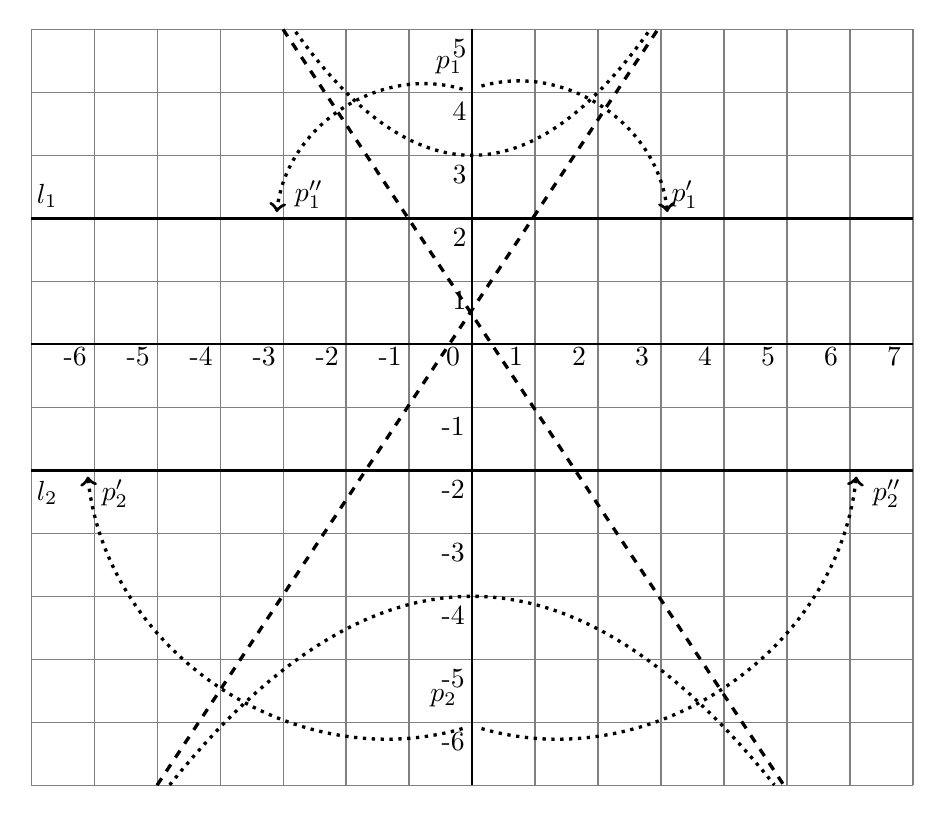
\begin{tikzpicture}[scale=.8]
\draw[step=10mm,white!50!black,thin] (-7,-7) grid (7,5);
\draw[thick] (-7,0) -- (7,0);
\draw[thick] (0,-7) -- (0,5);
\foreach \x in {-6,...,7}
  \node at (\x-.3,-.2) {\sm{\x}};
\foreach \y in {1,...,5}
  \node at (-.2,\y-.3) {\sm{\y}};
\foreach \y in {-6,...,-1}
  \node at (-.3,\y-.3) {\sm{\y}};
  
\coordinate (P1) at (0,4);
\coordinate (P2) at (0,-6);
\coordinate (P1P) at (3.1,2);
\coordinate (P2P) at (-6.12,-2);
\coordinate (P1PP) at (-3.1,2);
\coordinate (P2PP) at (6.12,-2);

\vertex{P1};
\vertex{P2};
\vertex{P1P};
\vertex{P2P};
\vertex{P1PP};
\vertex{P2PP};

\node[above left,yshift=3pt] at (P1) {$p_1$};
\node[above left,xshift=-2pt,yshift=2pt] at (P2) {$p_2$};
\node[above right,xshift=-2pt] at (P1P) {$p_1'$};
\node[below right,xshift=2pt] at (P2P) {$p_2'$};
\node[above right,xshift=3pt] at (P1PP) {$p_1''$};
\node[below right,xshift=2pt] at (P2PP) {$p_2''$};

\draw[very thick] (-7,2) -- node[very near start,above,xshift=-34pt] {$l_1$} (7,2);
\draw[very thick] (-7,-2) -- node[very near start,below,xshift=-34pt] {$l_2$} (7,-2);

\draw[domain=-4.8:4.8,samples=50,very thick,dotted] plot (\x,{-.13*\x*\x-4});
\draw[domain=-2.8:2.8,samples=50,very thick,dotted] plot (\x,{.25*\x*\x+3});

\draw[very thick,dashed] (-5,-7) -- (2.95,5);
\draw[very thick,dashed] (-3,5) -- (4.95,-7);

\draw[very thick,dotted,->,bend left=50] (.15,4.1) to (3.1,2.1);
\draw[very thick,dotted,->,bend right=50] (-.15,4.05) to (-3.1,2.1);

\draw[very thick,dotted,->,bend right=50] (.15,-6.1) to (6.1,-2.1);
\draw[very thick,dotted,->,bend left=50] (-.15,-6.1) to (-6.1,-2.1);

\end{tikzpicture}

\end{center}
\caption{אקסיומה 6}\label{f.axiom6}
\end{figure}

קיפול המניח את 
$p_i$
על
$l_i$
הוא קו
$l_f$
שהמרחק מ-%
$p_i$
ל-%
$l_f$
שווה למרחק מ-%
$l_i$
ל-%
$l_f$.
המקום הגיאומטרי של נקודות שהן במרחק שווה מנקודה
$p_i$
ומקו
$l_i$
הוא פרבולה עם מוקד 
\L{(focus)}
$p_i$
ומדריך
\L{(directrix)}
$l_i$.
קיפול הוא כל קו המשיק לפרבולה (סעיף~%
\ref{s.parabola}).

כדי שהקיפול יניח בו-זמנית את 
$p_1$
על ל-%
$l_1$
ו-%
$p_2$
על ל-%
$l_2$,
הוא חייב להיות משיק משותף לשתי הפרבולות. מספר המשיקים המשותפים הוא אפס, אחד, שניים או שלושה (איורים%
~\ref{f.two-para-1-zero}, 
\ref{f.two-para-1-one},
\ref{f.two-para-1-two}, 
\ref{f.two-para-1-three}).

הנוסחה של פרבולה שרירותית מסובכת מאוד ולנן נביא את הנוסחאות רק עבור פרבולות שציר הסמטריה הוא ציר ה-%
$x$
או ציר ה-%
$y$.
\begin{figure}[tb]
\begin{center}
\begin{subfigure}{.45\textwidth}
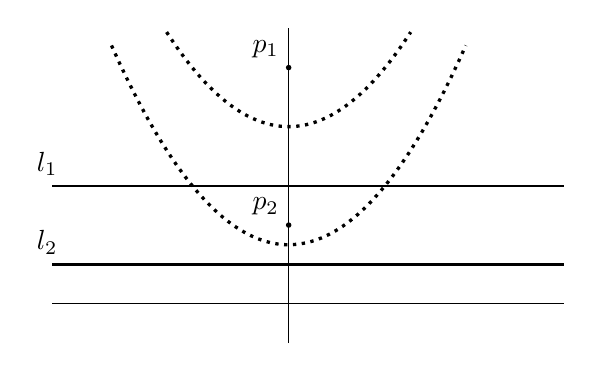
\begin{tikzpicture}[scale=.5]
\draw (-6,0) -- (7,0);
\draw (0,-1) -- (0,7);
\coordinate (P1) at (0,6);
\fill (P1) circle (2pt) node[above left] {$p_1$};
\coordinate (P2) at (0,2);
\fill (P2) circle (2pt) node[above left] {$p_2$};
\draw[thick] (-6,3) -- node[very near start,above,xshift=-25pt] {$l_1$} (7,3);
\draw[thick] (-6,1) -- node[very near start,above,xshift=-25pt] {$l_2$} (7,1);
\draw[domain=-3.1:3.1,samples=50,very thick,dotted] plot (\x,{.25*\x*\x+4.5});
\draw[domain=-4.5:4.5,samples=50,very thick,dotted] plot (\x,{.25*\x*\x+1.5});
\end{tikzpicture}
\caption{אפס משיקים}\label{f.two-para-1-zero}
\end{subfigure}
\hspace{2em}
\begin{subfigure}{.45\textwidth}
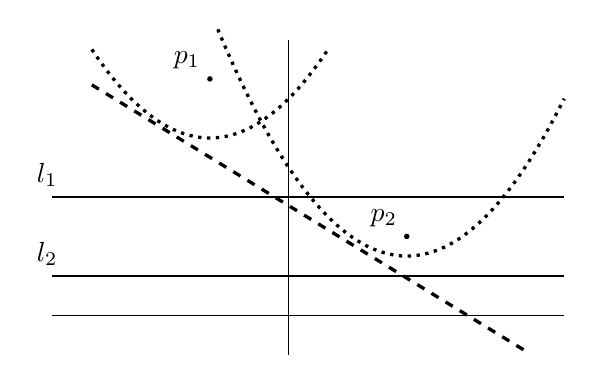
\begin{tikzpicture}[scale=.5]
\draw (-6,0) -- (7,0);
\draw (0,-1) -- (0,7);
\coordinate (P1) at (-2,6);
\fill (P1) circle (2pt) node[above left] {$p_1$};
\coordinate (P2) at (3,2);
\fill (P2) circle (2pt) node[above left] {$p_2$};
\draw[thick] (-6,3) -- node[very near start,above,xshift=-25pt] {$l_1$} (7,3);
\draw[thick] (-6,1) -- node[very near start,above,xshift=-25pt] {$l_2$} (7,1);
\draw[domain=-5:1,samples=50,very thick,dotted] plot (\x,{.25*(\x+2)*(\x+2)+4.5});
\draw[domain=-1.8:7,samples=50,very thick,dotted] plot (\x,{.25*(\x-3)*(\x-3)+1.5});
\draw[very thick,dashed] (-5,5.85) -- (6,-.9);
\end{tikzpicture}
\caption{משיק אחד}\label{f.two-para-1-one}
\end{subfigure}
\end{center}
\end{figure}

\begin{figure}[tb]
\begin{center}
\begin{subfigure}{.45\textwidth}
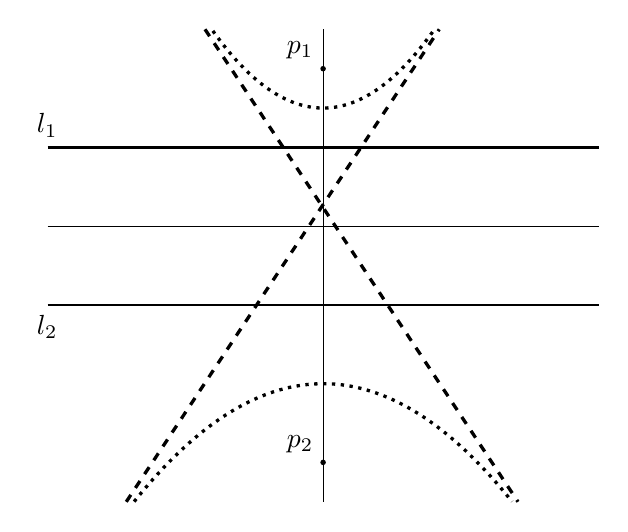
\begin{tikzpicture}[scale=.5]
\draw (-7,0) -- (7,0);
\draw (0,-7) -- (0,5);
\coordinate (P1) at (0,4);
\fill (P1) circle (2pt) node[above left] {$p_1$};
\coordinate (P2) at (0,-6);
\fill (P2) circle (2pt) node[above left] {$p_2$};
\draw[thick] (-7,2) -- node[very near start,above,xshift=-25pt] {$l_1$} (7,2);
\draw[thick] (-7,-2) -- node[very near start,below,xshift=-25pt] {$l_2$} (7,-2);
\draw[domain=-4.8:4.8,samples=50,very thick,dotted] plot (\x,{-.13*\x*\x-4});
\draw[domain=-2.8:2.8,samples=50,very thick,dotted] plot (\x,{.25*\x*\x+3});
\draw[very thick,dashed] (-5,-7) -- (2.95,5);
\draw[very thick,dashed] (-3,5) -- (4.95,-7);
\end{tikzpicture}
\selectlanguage{hebrew}
\caption{שני משיקים}\label{f.two-para-1-two}
\end{subfigure}
\hspace{2em}
\begin{subfigure}{.45\textwidth}
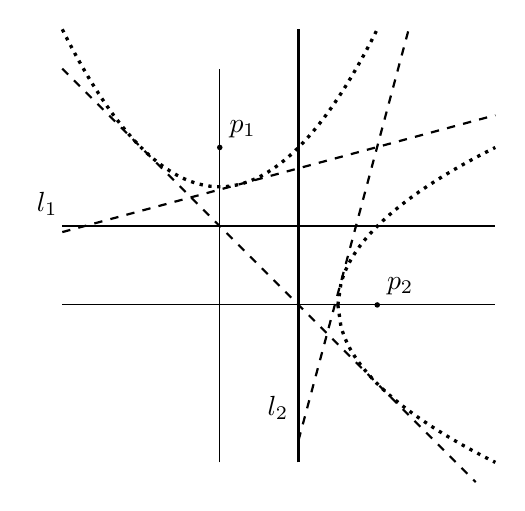
\begin{tikzpicture}[scale=.5]
\draw (-4,0) -- (7,0);
\draw (0,-4) -- (0,6);
\coordinate (P1) at (0,4);
\fill (P1) circle (2pt) node[above right] {$p_1$};
\coordinate (P2) at (4,0);
\fill (P2) circle (2pt) node[above right] {$p_2$};
\draw[thick] (-4,2) -- node[very near start,above,xshift=-25pt] {$l_1$} (7,2);
\draw[thick] (2,-4) -- node[very near start,left] {$l_2$} (2,7);
\draw[domain=-4:4,samples=50,very thick,dotted] plot (\x,{.25*\x*\x+3});
\draw[domain=3:7,samples=50,very thick,dotted] plot (\x,{sqrt(4*\x-12)});
\draw[domain=3:7,samples=50,very thick,dotted] plot (\x,{-sqrt(4*\x-12)});

\draw[thick,dashed,domain=-4:6.5] plot (\x,-\x+2);
\draw[thick,dashed,domain=-4:7] plot (\x,.27*\x+2.93);
\draw[thick,dashed,domain=2:4.8] plot (\x,3.73*\x-10.9);
\end{tikzpicture}
\selectlanguage{hebrew}
\caption{שלושה משיקים}\label{f.two-para-1-three}
\end{subfigure}
\end{center}
\end{figure}


\subsection{פיתוח הנקודה של הקיפול}

תהי הנקודה
$(0,f)$
מוקד של פרבולה עם מדריך
$y=d$.
נגדיר
$p=f-d$,
האורך עם סימן פלוס או מינוס של קטע הקו בין המוקד למדריך.%
\footnote{%
השתמשנו עד כה בסימון 
$p_i$
עבור נקודות. השימוש כאן ב-%
$p$
עלול לבלבל אבל ניסוח זה מקובל בספרות. השם הפורמלי עבור 
$p$
הוא מחצית ה-%
\L{latus rectum}.}
אם הקודקוד 
\L{(vertex)}
של הפרבולה נמצא על ציר ה-%
$x$,
המשוואה של הפרבולה היא
$y=\disfrac{x^2}{2p}$.
כדי להזיז את הפרבולה למעלה או למטה על ציר ה-%
$y$,
כדי שהקודקוד יהיה
$(0,h)$,
יש להוסיף 
$h$
למשוואת הפרבולה (איור%
~\ref{f.parabola}):
\[
y=\disfrac{x^2}{2p}+h\,.
\]
\begin{figure}[tb]
\begin{center}
\begin{tikzpicture}[scale=.8]
\draw (-6,0) -- node[very near start,below,xshift=-32pt] {$x$-\R{ציר}}(6,0);
\draw (0,-3) -- node[very near start,right,yshift=-20pt] {$y$-\R{ציר}}(0,4.5);
\draw[very thick] (-6,-2) -- node[near start,below] {\R{מדריך} $\quad y=-2$} (6,-2);
\draw[domain=-5:5,samples=50,very thick,dotted] plot (\x,{\x*\x/8+1});
\coordinate (F) at (0,4);
\fill (F) circle (2pt) node[left,xshift=-2pt,yshift=0pt] {$(0,f)=(0,4)$} node[above left,xshift=-2pt,yshift=4pt] {\R{מוקד}};
\fill (0,-2) circle (2pt);
\fill (0,1) circle (2pt) node[below left] {\R{קודקוד}} node[below left,yshift=-10pt] {$(0,1)$};
\draw[<->] (2,-1.9) -- node[fill=white] {$p=6$} +(0,5.8);
\draw[<->] (1,.1) -- node[fill=white] {$h=1$} +(0,.8);
\end{tikzpicture}
\end{center}
\selectlanguage{hebrew}
\caption{הגדרת הפרבולה: מוקד, מדריך, קודקוד}\label{f.parabola}
\end{figure}
נגדיר
$a=2ph$
כדי שמשוואת הפרבולה תהיה:
\begin{eqnlabels}
y&=&\disfrac{x^2}{2p}+\disfrac{a}{2p}\\
\label{eq.eq-parabola}x^2-2py+a&=&0\,.
\end{eqnlabels}
עבור הפרבולה באיור~%
\ref{f.parabola}
המשוואה היא
$x^2-12y +12=0$.

נציב את המשוואה של קו 
\textbf{שרירותי}
$y=mx+b$
במשוואה%
~\ref{eq.eq-parabola}
ונקבל משוואה עבור נקודות החיתוך של הקו והפרבולה:
\begin{eqn}
x^2-2p(mx+b)+a&=&0\\
x^2+(-2mp)x+(-2pb+a)&=&0\,.
\end{eqn}
הקו יהיה משיק לפרבולה אם ורק אם למשוואה ריבועית זו קיים 
\textbf{בדיוק}
פתרון אחד אם ורק אם הדיסקרימננטה 
(\L{discriminant})
היא אפס:
\begin{eqnlabels}
(-2mp)^2\:-\:4\cdot 1\cdot (-2pb+a)&=&0\\
m^2p^2+2pb-a&=&0\,.\label{eq.disc}
\end{eqnlabels}
משוואה זו עם המשתנים
$m$ 
היא המשוואה עבור המשיקים לפרבולה, אבל אנחנו מחפשים משיקים משותפים של שני משיקים, ולכן יש לפתור את המשוואות עבור שתי פרבולות.

%%%%%%%%%%%%%%%%%%%%%%%%%%%%%%%%%%%%%%%%%%%%%%%%%%%%%%%%%%%%%%%%

\begin{example}
\mbox{}\\
\textbf{פרבולה 1:}
מוקד
$(0,4)$,
מדריך
$y=2$,
קודקוד
$(0,3)$.


$p=4-2=2$, $a=2\cdot 2\cdot 3=12$.
משוואת הפרבולה היא:
\[
x^2-4y +12=0\,.
\]
נציב לתוך משוואה%
~\ref{eq.disc}
ונפשט:
\[
m^2+b-3=0\,.
\]
\textbf{פרבולה 2:}
מוקד
$(0,-4)$,
מדריך
$y=-2$,
קודקוד
$(0,-3)$.

$p=-4-(-2)=-2$, $a=2\cdot -2\cdot -3=12$.
משוואת הפרבולה היא:
\[
x^2+4y+12=0\,.
\]
נציב לתוך משווארה%
~\ref{eq.disc}
ונפשט:
\[
m^2-b-3=0\,.
\]
הפתרונות של שתי המשוואות:
\begin{eqn}
m^2+b-3&=&0\\
m^2-b-3&=&0\,,
\end{eqn}
הם
$m=\pm\sqrt{3}\approx \pm 1.73$
ו-%
$b=0$.
המשיקים המשותפים שהם הקיפולים הם:
\[
y=\sqrt{3}x\,,\quad y=-\sqrt{3}x\,.
\]
\end{example}

%%%%%%%%%%%%%%%%%%%%%%%%%%%%%%%%%%%%%%%%%%%%%%%%%%%%%%%%%%%%%%%%

\begin{example}
\mbox{}\\
\textbf{פרבולה 1:}
ללא שינוי.

\textbf{פרבולה 2:}
מוקד
$(0,-6)$,
מדריך
$y=-2$,
קודקוד
$(0,-4)$.

$p=-6-(-2)=-4$, $a=2\cdot -4\cdot -4=32$.
משוואת הפרבולה היא:
\[
x^2+8y +32=0\,.
\]
נציב לתוך משוואה%
~\ref{eq.disc}
ונפשט:
\[
2m^2-b-4=0\,.
\]
הפתרונות של שתי המשוואות:
\begin{eqn}
m^2+b-3&=&0\\
2m^2-b-4&=&0\,,
\end{eqn}
הם
$m=\pm\sqrt{\disfrac{7}{3}}\approx \pm 1.53$
ו-%
$b=\disfrac{2}{3}$.
יש שני משיקים משותפים שהם קיפולים:
\[
y=\sqrt{\disfrac{7}{3}}x+\disfrac{2}{3}\,,\quad y=-\sqrt{\disfrac{7}{3}}x+\disfrac{2}{3}\,.
\]
\end{example}

%%%%%%%%%%%%%%%%%%%%%%%%%%%%%%%%%%%%%%%%%%%%%%%%%%%%%%%%%%%%%%%%

\begin{example}
\mbox{}\\
עכשיו נגדיר פרבולה שציר הסמטריה שלה הוא ציר ה-%
$x$.

\textbf{פרבולה 1:}
ללא שינוי, המשוואה היא:
\[
m^2+b-3=0\,.
\]
\textbf{פרבולה 2:}
מוקד
$(4,0)$,
מדריך
$x=2$,
קודקוד
$(3,0)$.

$p=4-2=2$, $a=2\cdot 2\cdot 3=12$.
משוואת הפרבולה היא:
\begin{equation}
y^2-4x+12 = 0\,.\label{eq.x-symmetry-parabola}
\end{equation}
שימו לב שזו משוואה עם 
$x$
ו-%
$y^2$
במקום
$x^2$
ו-%
$y$,
כך שלא ניתן להשתמש במשוואה%
~\ref{eq.disc}
ונצטרך לפתח את משוואות מחדש.

נציב את המשוואה של הקו במשוואה%
~\ref{eq.x-symmetry-parabola}:
\begin{eqn}
(mx+b)^2-4x+12&=&0\\
m^2x^2+(2mb-4)x+(b^2+12)&=&0\,
\end{eqn}
נשווה את הדיסקרימננטה לאפס ונפשט:
\begin{eqn}
(2mb-4)^2\:-\:4m^2(b^2+12)&=&0\\
-3m^2-mb+1&=&0\,.
\end{eqn}
אם ננסה לפתור את שתי המשוואות:
\begin{eqn}
m^2+b-3&=&0\\
-3m^2-mb+1&=&0\,,
\end{eqn}
נקבל משוואה 
\textbf{ממעלה שלוש}
במשתנה
$m$:
\begin{equation}
m^3-3m^2-3m+1=0\,.\label{eq.cubic}
\end{equation}
למשוואה ממעלה שלוש יש לפחות פתרון ממשי אחד ולכל היותר שלושה פתרונות ממשיים, לכן יכול להיות אחד, שניים או שלשה משיקים משותפים. הנוסחה למציאת פתרונות למשוואה ממעלה שלוש די מסובכת, לכן השתמשתי במחשבון באינטרנט וקיבלתי שלושה פתרונות:
\[
m=3.73\,, \;m=-1\,, \; m=0.27\,.
\]
מהצורה של המשוואה%
~\ref{eq.cubic},
נוכל לנחש ש-%
$1$
או
$-1$
הוא פתרון:
\begin{eqn}
1^3-3\cdot 1^2-3\cdot 1+1&=&-4\\
(-1)^3-3\cdot (-1)^2-3\cdot(-1)+1&=&0\,.
\end{eqn}
נחלק את המשוואה%
~\ref{eq.cubic}
ב-%
$m-(-1)=m+1$
ונקבל משוואה ריבועית
$m^2-4m+1$
ששורשיה הם
$2\pm\sqrt{3}\approx 3.73, 0.27$.
\end{example}

%%%%%%%%%%%%%%%%%%%%%%%%%%%%%%%%%%%%%%%%%%%%%%%%%%%%%%%%%%%%%%%%

\subsection{פיתוח המשוואות של השיקופים}

נחשב את  
$p_1'=(x_1',y_1')$,
השיקוף של
$p_1=(x_1,y_1)$
מסביב למשיק
$l_t$
שהמשוואה שלה היא
$y=m_tx+b_t$.
תחילה, נמצא את הקו
$l_p$
עם המשוואה
$y=m_px+b_p$
שניצב ל-%
$l_t$
ועובר דרך
$p_1$:
\begin{eqn}
y&=&-\disfrac{1}{m_t}x+b_p\\
y_1&=&-\disfrac{1}{m_t}x_1+b_p\\
y&=&\disfrac{-x}{m_t}+\left(y_1+\disfrac{x_1}{m_t}\right)\,.
\end{eqn}
כעת נמצא את נקודת החיתוך 
$p_t=(x_t,y_t)$
של
$l_t$
ו-%
$l_p$:
\begin{eqn}
m_tx_t+b_t&=&\frac{-x_t}{m_t}+\left(y_1+\frac{x_1}{m_t}\right)\\
x_t&=&\frac{\left(y_1+\displaystyle\frac{x_1}{m_t}-b_t\right)}{\left(m_t+\displaystyle\frac{1}{m_t}\right)}\\
y_t&=&m_tx_t+b_t\,.
\end{eqn}
$p_t$
היא נקודה האמצע בין 
$p_1$

ל-%
$p_1'$:
\[
\begin{array}{rcl@{\hspace{3ex}}rcl}
x_t&=&\displaystyle\frac{x_1+x_1'}{2}\,, &x_1'&=&2x_t-x_1\,,\\
y_t&=&\displaystyle\frac{y_1+y_1'}{2}\,,& y_1'&=&2y_t-y_1\,.
\end{array}
\]
\begin{example}
יהי
$l_t$
הקו
$y=\sqrt{3}x+0$
ו-%
$p_1=(0,4)$:
\begin{eqn}
x_t&=&\frac{\left(4+\displaystyle\frac{0}{\sqrt{3}}-0\right)}{\left(\sqrt{3}+\displaystyle\frac{1}{\sqrt{3}}\right)}=\sqrt{3}\\
y_t&=&\sqrt{3}\sqrt{3}+0=3\\
x_1'&=&2x_t-x_1=2\sqrt{3}\approx 3.46\\
y_1'&=&2y_t-y_1= 2\,.
\end{eqn}

\end{example}

%%%%%%%%%%%%%%%%%%%%%%%%%%%%%%%%%%%%%%%%%%%%%%%%%%%%%%%

\newpage

\subsection{משיקים לפרבולה}\label{s.parabola}

אנו רוצים להוכיח שהקיפולים של אקסיומה
$6$
הם משיקים לפרבולות. איור~%
\ref{f.para:locus}
מראה חמש נקודות
$p_1,\ldots,p_5$,
על הפרבולה כאשר כל נקודה
$p_i$
היא במרחק
$a_i$
גם מהמוקד וגם מהמדריך. נוריד ניצבים למדריך מ-%
$p_i$,
ונסמן ב-%
$p_i'$
את נקודות החיתוך של הניצב עם המדריך. לפי אקסיומה $2$ קיימים קיפולים 
$l_i$
דרך
$p_i$
שמניח את 
$p$
המדריך. האיור מראה את הקיפול 
$l_1$
דרך 
$p_1$
ואת השיקוף
$p_1'$.

\begin{figure}[tb]
\begin{center}
\begin{tikzpicture}[scale=.8]
\draw (-6,0) -- node[very near start,below,xshift=-32pt] {$x$%
\R{ציר ה-}}
(6,0);
\draw (0,-3.2) -- node[very near start,right,yshift=-20pt] {$y$%
\R{ציר ה-}}
(0,4.5);
\draw[thick] (-6,-2) -- node[near end,below] {\R{מדריך} $\quad y=-f$} (6,-2);
\draw[domain=-6:6,samples=50,very thick,dotted] plot (\x,{\x*\x/8});
\coordinate (F) at (0,2);
\vertex{F};
\node[above left,xshift=-2pt,yshift=15pt] at (F) {$(0,f)$};
\node[above left,xshift=-5pt,yshift=30pt] at (F) {\R{מוקד}}; \node[above right] at (F) {$p$};
\coordinate (vertex) at (0,0);
\vertex{vertex};
\node[below right] at (vertex) {$p_2$};
\coordinate (FP) at (-5,-2);
\node[below] at (FP) {$p_1'$};
\coordinate (F1) at (2,.5);
\vertex{F1};
\node[below right] at (F1) {$p_3$};
\coordinate (F2) at (3,1.125);
\vertex{F2};
\node[below right] at (F2) {$p_4$};
\coordinate (F3) at (5,3.125);
\vertex{F3};
\node[below right] at (F3) {$p_5$};
\coordinate (F4) at (-5,3.125);
\vertex{F4};
\node[above right] at (F4) {$p_1$};
\draw (F) -- node[left] {$a_2$} (0,0) -- node[left] {$a_2$} (0,-2);
\draw (F) -- node[near end,left] {$a_3$} (F1) -- node[left] {$a_3$} (2,-2);
\draw (F) -- node[near end,above] {$a_4$} (F2) -- node[left] {$a_4$} (3,-2);
\draw (F) -- node[above] {$a_5$} (F3) -- node[left] {$a_5$} (5,-2);
\draw (F) -- node[above] {$a_1$} (F4) -- node[left] {$a_1$} (FP);
\draw[very thick,dashed] ($(F4)!-.4!(-2.5,0)$) -- node[near end,right,xshift=2pt] {$l_1$} ($(F4)!1.8!(-2.5,0)$);
\draw (0,-2) rectangle +(9pt,9pt);
\draw (2,-2) rectangle +(9pt,9pt);
\draw (3,-2) rectangle +(9pt,9pt);
\draw (5,-2) rectangle +(9pt,9pt);
\draw (-5,-2) rectangle +(9pt,9pt);
\end{tikzpicture}
\end{center}
\caption{המשיק כמקום הגיאומטרית}\label{f.para:locus}
\end{figure}

\begin{theorem}\label{thm.parabola-tangents}
הקיפולים של אקסיומה
$6$
הם משיקים לפרבולה והמקומות הגיאומטריים של הנקודות שהן במרחק שווה מ-%
$p_1,p_2$
ומ-%
$l_1,l_2$,
בהתאמה.
\end{theorem}

\begin{proof}
באיור~%
\ref{f.tangent-proof}
המוקד הוא 
$p$,
המדריך הוא 
$l$,
$p'$
היא נקודה על המדריך, ו-%
$l$
הוא הקיפול המשקף את
$p$
על 
$p'$.
תהי 
$s$
נקודת החיתוך של 
$\overline{pp'}$
ו-%
$l$.
אזי 
$\overline{ps}=\overline{p's}=a$
ו-%
$l\perp \overline{pp'}$.

\begin{figure}[tb]
\begin{center}
\begin{tikzpicture}[scale=.8]
\draw[thick] (-6,-2) -- node[near end, below] {$d$} (6,-2);
\draw[domain=-5.5:5.5,samples=50,very thick,dotted] plot (\x,{\x*\x/8});
\coordinate (F) at (0,2);
\vertex{F};
\node[above right] at (F) {$p$};
\coordinate (FP) at (-3,-2);
\node[below] at (FP) {$p'$};
\coordinate (F4) at (-3,1.125);
\vertex{F4};
\node[above right] at (F4) {$r$};
\coordinate (F5) at (-5,2.775);
\vertex{F5};
\node[left,yshift=-4pt] at (F5) {$q$};
\coordinate (F5p) at (-5,-2);
\node[below] at (F5p) {$p''$};
\draw (F) -- node[above] {$b$} (F4) -- node[left] {$b$} (FP);
\draw (F) -- node[above] {$c$} (F5);
\draw (F5) -- node[left] {$e$} (F5p);
\draw[thick,dashed,name path=fold] ($(F4)+(140:4)$) -- (F4) -- node[below,xshift=3pt,yshift=-4pt] {$l$} ($(F4)+(-40:5.3)$);
\draw (FP) rectangle +(10pt,10pt);
\draw (F5p) rectangle +(10pt,10pt);
\draw (F5) -- (FP);
\draw[name path=base] (F) -- (FP);
\path [name intersections = {of = base and fold, by = {G}}];
\node[below,yshift=-4pt] at (G) {$s$};
\draw[rotate=140] (G) rectangle +(10pt,10pt);
\path (FP) -- node[left] {$c$} (F5);
\path (F) -- node[below] {$a$} (G) -- node[below] {$a$} (FP);
\end{tikzpicture}
\end{center}
\caption{ההוכחה שקיפול הוא משיק}\label{f.tangent-proof}
\end{figure}
תהי
$r$
נקודת החיתוך של הניצב ל-%
$d$
דרך 
$p'$
והקיפול
$l$.
אזי
$\triangle psr\cong \triangle p'sr$
לפי צלע-זווית-צלע. מכאן ש-%
$\overline{pr}\!=\!\overline{p'r}\!=\!b$
ולכן
$r$
נמצאת על הפרבולה. נבחר נקודה
$p''$
שונה מ-%
$p'$
על המדריך ונניח שהקיפול
$l$
משקף גם את
$p$ 
על
$p''$.
תהי 
$q$
החיתוך של הניצב ל-%
$d$
דרך 
$p''$
והקיפול
$l$.
$\triangle psq\cong \triangle p'sq$ 
ןלכן
$\overline{pq}\!=\!\overline{p'q}\!=\!c$.
נסמן
$\overline{qp''}\!=\!e$.
אם
$q$
נמצאת על הפרבולה, אזי
$e\!=\!\overline{qp''}\!=\!\overline{qp}\!=\!c$,
אבל
$c$
הוא היתר של המשולש ישר-זווית
$\triangle qp''p'$
ולא ייתכן שהיתר שווה לאחת הצלעות של המשולש. לכן לקיפול
$l$
נקודת חיתוך אחת עם בפרבולה והוא הקיפול הוא משיק.
\end{proof}

%%%%%%%%%%%%%%%%%%%%%%%%%%%%%%%%%%%%%%%%%%%%%%%%%%%%%%%%%%%%%%%%

\newpage

\section{אקסיומה 7}\label{s.ax7}

\begin{axiom}
נתונה נקודה 
$p_1=(x_1,y_1)$,
ונתונים קווים
$l_1$
ו-%
$l_2$,
קיים קיפול
$l$
הניצב ל-%
$l_2$
שהמניח את
$p_1$
על ל-%
$l_1$
(איור~%
\ref{f.axiom7}).
\end{axiom}

\begin{figure}[tb]
\begin{center}

\begin{tikzpicture}[scale=.9]
\draw[step=10mm,white!50!black,thin] (-1,-1) grid (9,8);
\draw[thick] (-1,0) -- (9,0);
\draw[thick] (0,-1) -- (0,8);
\foreach \x in {0,...,9}
  \node at (\x-.2,-.2) {\sm{\x}};
\foreach \y in {1,...,8}
  \node at (-.2,\y-.3) {\sm{\y}};
  
\coordinate (P1) at (5,3);
\fill (P1) circle (2pt) node[below left] {$p_1$};

\coordinate (P1P) at (2.75,5.25);
\fill (P1P) circle (2pt) node[left,xshift=-4pt] {$p_1'$};

\draw[very thick] (1,0) -- node[very near start,right,xshift=2pt] {$l_1$} (3,6);
\draw[very thick,name path=l2] (8,3) -- node[very near start,right,xshift=-2pt,yshift=6pt] {$l_2$} (5,6);

\draw[thick,dotted] ($(1,0)!-.15!(3,6)$) -- ($(1,0)!1.34!(3,6)$);

\draw[thick,dotted] ($(8,3)!-.3!(5,6)$) -- ($(8,3)!1.65!(5,6)$);

\draw[thick,dotted] ($(P1)!-.4!(P1P)$) -- node[very near start,below,yshift=-4pt] {$l_p$} ($(P1)!1.5!(P1P)$);

\draw[very thick,dashed,name path=fold] (-.5,-.25) -- node[very near end,above,xshift=4pt,yshift=6pt] {$l$} (7.5,7.75);

\coordinate (mid) at ($(P1)!.5!(P1P)$);
\fill (mid) circle (2pt) node[below,yshift=-8pt] {$p_m$};

\path [name intersections = {of = fold and l2, by = {perp}}];
\draw[rotate=-45] (mid) rectangle +(8pt,8pt);
\draw[rotate=-45] (perp) rectangle +(8pt,8pt);


\draw[very thick,dotted,->,bend right=50] (5.1,3.2) to (3,5.2);
\end{tikzpicture}
\end{center}
\caption{אקסיומה 7}\label{f.axiom7}
\end{figure}

הקיפול הוא המקום הגיאומטרי של כל הנקודות על הקו הניצב ל-%
$l_2$
ושנמצא במרחק שווה מ-%
$p_1$
ו-%
$p_1'$,
השיקוף של
$p_1$
על
$l_1$.

\textbf{פיתוח משוואת הקיפול:}
תהי
$p_1=(x_1,y_1)$,
יהי
$l_1$
הקו
$y = m_1x + b_1$ 
ו-%
$l_2$
הקו
$y=m_2x+b_2$.
יהי
$l_p$
הקו שמכיל את
$\overline{p_1p_1'}$.
מ-%
$l\perp l_2,l_p\perp l$
נובע ש-%
$l_p\parallel l_2$
והמשוואה של
$l_p$
היא
$y=m_2x+b_p$.

$l_p$
עובר דרך
$p_1$
ולכן
$y_1=m_2x_1+b_p$
והמשוואה שלו היא
$y=m_2x+(y_1-m_2x_1)$.
השיקוף 
$p_1'=(x_1',y_1')$
הוא נקודת החיתוך של
$l_1$
ו-%
$l_p$:
\begin{eqn}
m_1x_1'+b_1&=&m_2x_1'+(y_1-m_2x_1)\\
x_1'&=&\disfrac{y_1-m_2x_1-b_1}{m_1-m_2}\\
y_1'&=&m_1x_i'+b_1\,.
\end{eqn}
$p_m=(x_m,y_m)$,
נקודת האמצע של
$l_p$,
היא:
\[
(x_m,y_m)=\left(\disfrac{x_1+x_1'}{2},\disfrac{y_1+y_1'}{2}\right)\,.
\]
$l\perp l_2$
ועבור דרך
$p_m$
ולכן המשוואה שלו היא:
\[
y_m=-\disfrac{1}{m_2}x_m+b_m\,.
\]
כאשר ניתן לחשב את 
$b_m$
מ-%
$y=-\displaystyle\frac{1}{m_2}x+b_m$:
\[
b_m=y_m+\disfrac{x_m}{m_2}\,.
\]
המשוואה של הקיפול
$l$
היא:
\[
y=-\disfrac{1}{m_2}x+\left(y_m+\disfrac{x_m}{m_2}\right)\,.
\]
\begin{example}
נתונה הנקודה
$p_1=(5,3)$,
נתון הקו 
$l_1$
שהמשוואה שלו היא
$y=3x-3$,
ונתון הקו
$l_2$
שהמשוואה שלו היא
$y=-x+11$.
אזי:
\begin{eqn}
x_1'&=&\disfrac{3-(-1)\cdot 5-(-3)}{3-(-1)}=\disfrac{11}{4}\\
y_1' &=&3\cdot\disfrac{11}{4} + (-3)=\disfrac{21}{4}\\
	p_m&=&\left(\disfrac{5+\disfrac{11}{4}}{2},\disfrac{3+\disfrac{21}{4}}{2}\right)=\left(\disfrac{31}{8},\disfrac{33}{8}\right)\,.
\end{eqn}
משוואת הקיפול היא:
\[
y=-\disfrac{1}{-1}\cdot x+\left(\disfrac{33}{8}+\disfrac{\disfrac{31}{8}}{-1}\right)=x+\disfrac{1}{4}\,.
\]
\end{example}

%%%%%%%%%%%%%%%%%%%%%%%%%%%%%%%%%%%%%%%%%%%%%%%%%%%

\subsection*{מה ההפתעה?}

אוריגמי, האומנות של קיפולי נייר, קיים מאות שנים, ולכן מפתיע שרק במאה העשרים פותחה הפורמליזציה שלו. מפתיע עוד יותר שקיים אקסיומתיזציה של קיפולי נייר. המתמטיקה של אורגמי היא דרך מצויינת ללמוד גיאומטריה אנליטית, תכונות של פרבולות והמושג מקום גיאומטרי.

\subsection*{מקורות}

ניתן למוצא את האקסיומות של אוריגמי ב-%
\cite{wiki:hh-axioms}.
\L{Lang}
\cite{lang}
מביא דוגמאות של יצירות אוריגמי. פרק%
~$10$
של
\cite{martin}
מציג את התיאוריה המפורטת של אורגמי, כולל הוכחה שלפרבולה יכולה להיות אפס, אחד, שניים או שלושה משיקים. אוריה בן-לולו הראתה לי את ההוכחה של משפט%
~\ref{thm.parabola-tangents}.
מצאתי שתוכנה גיאומטרית כגון 
\L{Geogebra}
עוזרת להבין את הקשר בין הגיאומטריה והאלגברה של האקסיומות.

הצגה ברורה של משוואות קוביות ניתן למצוא בפרקים
$1,2$
של
\cite{jorg}.
